% =============================================================
% Capítulo 2 — Fundamentação Teórica
% =============================================================

\chapter{Fundamentação Teórica}\label{chap:fundamentacao_teorica}

\adicionadomarcelo{Este capítulo apresenta os conceitos necessários para a compreensão do trabalho. Inicialmente, são introduzidos fundamentos de aprendizado profundo e redes neurais artificiais, seguidos pelo processo de treinamento dessas redes. Em seguida, discute-se o problema do consumo energético em modelos de \textit{Deep Learning} e, por fim, são apresentadas as técnicas de compressão de modelos, com destaque para a poda neural (\textit{pruning}), que é o foco deste trabalho.}

A exposição é deliberadamente progressiva e não pressupõe familiaridade prévia com
aprendizado de máquina. Cada conceito é introduzido primeiro por meio de uma analogia com
situações cotidianas e só então formalizado, de modo que o leitor possa acompanhar o
raciocínio antes de encontrar a notação matemática que o descreve.

\section{Aprendizado Profundo e Redes Neurais}

\subsection{Aprendizado Profundo (Deep Learning)}
O Aprendizado Profundo é um campo especializado de aprendizado de máquina \adicionadomarcelo{\cite{Goodfellow2016,LeCun2015}}, \modificado{caracterizado pelo uso de redes neurais artificiais com múltiplas camadas, o que permite aprender e extrair informações complexas a partir de grandes volumes de dados}.

\subsection{Redes Neurais Artificiais}
\modificado{A rede neural artificial é um modelo computacional inspirado na estrutura do cérebro humano, que busca imitar a forma como neurônios se conectam e processam sinais para aprender a partir de dados, identificando padrões e tomando decisões. Um exemplo clássico é o perceptron multicamadas (MLP), um modelo composto por funções matemáticas que mapeiam valores de entrada em valores de saída \cite{Goodfellow2016}. Em tarefas de visão computacional, por exemplo, milhões de imagens de um objeto podem ser processadas para que a rede aprenda suas características visuais e seja capaz de reconhecê-lo posteriormente.}

Uma forma de tentar enteder a definição de uma RNN é, imagine uma comissão
encarregada de decidir se um pedido de empréstimo deve ser aprovado. Nenhum membro decide
sozinho, cada um examina um aspecto diferentee, como a renda declarada, o histórico de
pagamentos, o tempo de emprego e então, após analisar todos os aspectos, emite um parecer. Esses pareceres não têm todos o
mesmo valor, pois a comissão confia mais em uns avaliadores do que em outros, e a decisão
final combina todos eles, ponderados por essa confiança. Em uma rede neural, cada nó é um
desses avaliadores e o peso de cada conexão é exatamente a confiança depositada naquele
parecer. A diferença essencial é que a rede não recebe essas confianças prontas, ela as
descobre sozinha, por tentativa e erro, ao longo do treinamento.

Uma rede neural profunda é composta por unidades (nós) interconectadas, organizadas em camadas
\cite{Goodfellow2016,NielsenNNDL2015}.

\begin{itemize}
    \item \textbf{Nó (neurônio):} É uma unidade computacional que calcula uma soma ponderada das entradas mais um \textit{bias} e passa o resultado através de uma função de ativação, produzindo uma saída.
    \item \textbf{Camada de Entrada (Input Layer):} É onde o processo é iniciado e os dados são introduzidos na rede. O número de nós nessa camada corresponde ao número de características dos dados de entrada.
    \item \textbf{Camadas Ocultas (Hidden Layers):} São camadas intermediárias entre a entrada e a saída. Cada nó de uma camada oculta está conectado a todos os nós das camadas anterior e seguinte. É nelas que ocorre a maior parte do processamento e do aprendizado; a saída de uma camada oculta é utilizada como entrada da próxima, e, a cada camada, a rede passa a detectar características mais complexas e abstratas. Redes com múltiplas camadas ocultas são as chamadas redes de \textit{Deep Learning}.
    \item \textbf{Camada de Saída (Output Layer):} Camada final da rede, onde o resultado é produzido. A estrutura da camada de saída depende da tarefa: em regressão, há um único nó com função de ativação linear; em classificação binária, um único nó expressa resultados do tipo sim/não; em classificação multiclasse, há um nó para cada classe possível, e o de maior ativação corresponde à predição final.
\end{itemize}

\modificado{Cada conexão entre nós possui um peso associado, que determina a sua importância relativa. Pesos altos amplificam o sinal de entrada, enquanto pesos próximos de zero tornam a conexão pouco influente. Os pesos são inicializados com valores aleatórios e ajustados durante o treinamento \cite{Goodfellow2016}.}

% \begin{figure}[htb]
% \centering
% \caption{\adicionadomarcelo{Arquitetura típica de uma rede neural artificial com uma camada de entrada, duas camadas ocultas e uma camada de saída.}}
% \label{fig:arquitetura_rede_neural}
% 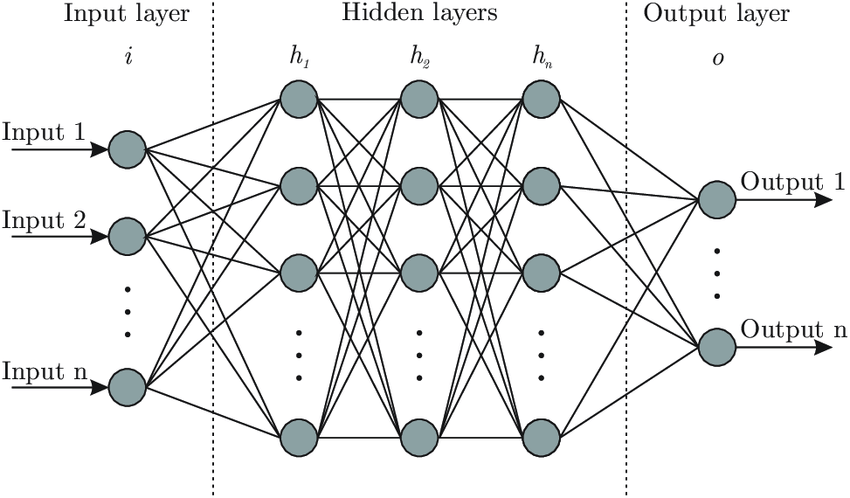
\includegraphics[scale=0.45]{02_capitulo/imageArquiteturaRedeNeural.png}
% % \\ \adicionadomarcelo{Fonte: \citeonline{NielsenNNDL2015}.}
% \end{figure}

\subsection{Bias em Redes Neurais}
\modificado{O \textit{bias} é um parâmetro adicional que ajusta a saída de um neurônio. Trata-se de um valor numérico associado a cada neurônio, não ligado a nenhuma entrada específica, atuando como um coeficiente linear. Antes da aplicação da função de ativação, o \textit{bias} é somado ao resultado da soma ponderada das entradas.}

A principal função do \textit{bias} é deslocar a função de ativação, permitindo que o modelo se ajuste melhor aos dados. Sem ele, a soma ponderada precisaria ser alta para que o neurônio fosse ativado; com o \textit{bias}, um neurônio pode ser ativado mesmo com uma soma ponderada baixa, caso seu \textit{bias} seja suficientemente alto \cite{NielsenNNDL2015}. Inversamente, um \textit{bias} muito negativo dificulta a ativação do neurônio. \modificado{O \textit{bias} é um parâmetro aprendível: inicialmente é inicializado com zero ou valores próximos de zero e, durante o treinamento, é atualizado pelo mesmo processo de retropropagação e descida de gradiente utilizado para os pesos.}

Retomando com a analogia da comissão de crédito, se os pesos representam o quanto se confia em cada
avaliador, o \textit{bias} representa o quanto o avaliador é exigente. Um membro
gentil aprova o pedido mesmo diante de evidências modestas; um membro rigoroso só
aprova quando as evidências são fortes. São duas coisas independentes --- confiar muito em
alguém não diz nada sobre o quanto essa pessoa é exigente --- e é por isso que a rede
precisa aprender os dois conjuntos de valores separadamente.

\subsection{Função de Ativação}
\modificado{A função de ativação é uma função matemática aplicada ao resultado da soma ponderada das entradas de um neurônio (já acrescido do \textit{bias}), determinando a saída do neurônio. Sua principal função é introduzir não linearidade no modelo: sem ela, a composição de diversas camadas resultaria em uma transformação puramente linear, equivalente a uma rede com uma única camada, o que limitaria drasticamente a capacidade expressiva do modelo \cite{Goodfellow2016}.}

A razão de existir dessa função merece um exemplo concreto, pois é ela que justifica o
próprio empilhamento de camadas. Considere um produto de R\$ 100,00 submetido a dois
descontos sucessivos, um de 10\% e outro de 20\%: o primeiro leva o preço a R\$ 90,00 e o
segundo a R\$ 72,00, exatamente o mesmo resultado que um único desconto de 28\% produziria.
Os dois passos colapsaram em um só, e o segundo nada acrescentou que um único desconto bem
escolhido não fizesse sozinho. Encadear operações lineares nunca gera nada além de outra
operação linear, e com redes neurais acontece o mesmo: sem função de ativação, uma rede de
cem camadas calcularia exatamente aquilo que uma única camada já calcularia, e toda a
profundidade seria desperdiçada.

Suponha agora que a loja adote uma regra adicional, aplicada logo depois de cada desconto:
nenhum produto pode ser vendido por menos de R\$ 85,00. Essa regra é o análogo da função de
ativação --- ela não faz parte do desconto, mas incide sobre o resultado dele, antes que
esse resultado siga para a etapa seguinte. Com ela, o encadeamento deixa de colapsar. O
produto de R\$ 100,00 cai para R\$ 90,00 e depois para R\$ 72,00, mas a regra o devolve a
R\$ 85,00, de modo que o desconto efetivo foi de 15\%. Já um produto de R\$ 200,00 percorre
os mesmos dois descontos, chega a R\$ 144,00 sem nunca esbarrar no limite e tem desconto
efetivo de 28\%. A mesma sequência de operações passou a produzir resultados diferentes
conforme a entrada, e nenhum desconto único reproduz esse comportamento. É esse
rompimento do encadeamento que permite a cada camada acrescentar algo que a anterior não
conseguia representar. A regra de preço mínimo, aliás, tem a mesma forma da ReLU,
apresentada adiante nesta seção: ambas preservam os valores acima de um limiar e
substituem os demais por um valor fixo.

A ativação de um neurônio ocorre em três etapas \cite{NielsenNNDL2015}:
\begin{itemize}
    \item \modificado{Soma ponderada: o neurônio multiplica o valor de ativação de cada nó da camada anterior pelo peso da respectiva conexão e soma todos os resultados.}
    \item \modificado{Adição do \textit{bias}: ao resultado da soma ponderada é somado o valor do \textit{bias}, que auxilia o neurônio a ativar-se mais ou menos facilidade.}
    \item \modificado{Função de ativação: o resultado final (soma ponderada acrescida do \textit{bias}) é passado pela função de ativação, cuja saída é então transmitida aos nós da próxima camada.}
\end{itemize}

\begin{figure}[htb]
\centering
\caption{\adicionadomarcelo{Representação matricial da propagação de um neurônio, da soma ponderada à função de ativação (Sigmoide).}}
\label{fig:matrizes_sigmoid}
\begin{tikzpicture}[font=\small]
  \node at (0,0) {$
    \underbrace{\begin{bmatrix} a_1 \\ a_2 \\ \vdots \\ a_m \end{bmatrix}}_{\substack{\text{ativações}\\\text{de saída}}}
    \;=\; \sigma\!\left(
    \underbrace{\begin{bmatrix}
      w_{11} & w_{12} & \cdots & w_{1n} \\
      w_{21} & w_{22} & \cdots & w_{2n} \\
      \vdots & \vdots & \ddots & \vdots \\
      w_{m1} & w_{m2} & \cdots & w_{mn}
    \end{bmatrix}}_{\text{pesos } W}
    \underbrace{\begin{bmatrix} x_1 \\ x_2 \\ \vdots \\ x_n \end{bmatrix}}_{\substack{\text{entradas da}\\\text{camada anterior}}}
    \;+\;
    \underbrace{\begin{bmatrix} b_1 \\ b_2 \\ \vdots \\ b_m \end{bmatrix}}_{\textit{bias}}
    \right)$};
  \begin{scope}[shift={(0,-3.5)}, scale=0.8]
    \draw[->] (-3.4,0) -- (3.6,0) node[right,font=\scriptsize] {$z$};
    \draw[->] (0,-0.3) -- (0,1.6) node[above,font=\scriptsize] {$\sigma(z)$};
    \draw[dashed,gray!70] (-3.4,1) -- (3.4,1);
    \node[font=\scriptsize,left] at (-0.1,1.05) {1};
    \node[font=\scriptsize,below left] at (0,0) {0};
    \draw[very thick] plot[domain=-3.4:3.4,samples=90] (\x,{1/(1+exp(-2*\x))});
    \node[font=\scriptsize,align=center] at (0,-1.0)
      {a função de ativação comprime qualquer valor de $z$ no intervalo $(0,1)$};
  \end{scope}
\end{tikzpicture}
\fonte{Adaptado de \citeonline{NielsenNNDL2015}.}
\end{figure}

Há diversas funções de ativação, cada uma com suas próprias características e aplicações.
\begin{itemize}
    \item \textbf{ReLU (Rectified Linear Unit):} \modificado{Função de ativação mais utilizada em redes neurais modernas, proposta para redes profundas por \citeonline{Nair2010} e popularizada por \citeonline{Krizhevsky2012}. É uma função linear por partes, com inclinação 1 para valores positivos e 0 para valores negativos. É computacionalmente muito eficiente e não sofre do problema do desaparecimento do gradiente para entradas positivas. Em contrapartida, pode sofrer do problema conhecido como \textit{Dying ReLU}, no qual neurônios cujas entradas se tornam persistentemente negativas deixam de ser ativados e param de aprender.}
    \item \textbf{Sigmoide:} \modificado{Função que mapeia qualquer valor real para o intervalo $(0,1)$, sendo útil em classificação binária, já que a saída pode ser interpretada como uma probabilidade. Caiu em desuso em camadas ocultas porque, para entradas com magnitude muito alta ou muito baixa, sua derivada se aproxima de zero, fenômeno conhecido como desaparecimento do gradiente \cite{Bengio1994}.}
    \item \textbf{Tanh (Tangente Hiperbólica):} \modificado{Semelhante à Sigmoide, porém mapeando os valores para o intervalo $(-1,1)$, o que a torna centrada em zero e costuma favorecer a convergência. Também sofre do problema do desaparecimento do gradiente.}
    \item \textbf{Softmax:} \modificado{Diferentemente das demais, não é aplicada a neurônios individuais de camadas ocultas, mas sim ao conjunto dos neurônios da camada de saída em tarefas de classificação multiclasse. Transforma as saídas brutas da última camada em uma distribuição de probabilidades, com valores no intervalo $(0,1)$ que somam 1. Na prática, converte pontuações sem escala definida em porcentagens comparáveis: o modelo deixa de responder ``7,2 para gato e 3,1 para cachorro'' e passa a responder ``85\% de chance de ser gato, 15\% de ser cachorro''.}
\end{itemize}

\modificado{Em cada camada, as ativações produzidas determinam as ativações da camada seguinte. De camada em camada, esses padrões tornam-se progressivamente mais complexos e abstratos, até que a camada de saída produz o resultado final. Assim, camadas iniciais aprendem características simples, enquanto camadas mais profundas combinam essas características para representar conceitos de alto nível \cite{LeCun2015}.}

\section{Treinamento de Redes Neurais}

\subsection{Gradiente}
\modificado{No contexto de redes neurais, o gradiente corresponde ao vetor de derivadas parciais da função de perda em relação aos pesos da rede. Ele é o elemento central que permite a minimização da função de perda por meio do algoritmo da descida do gradiente, um método de primeira ordem que utiliza as informações do gradiente para atualizar os parâmetros da rede \cite{Goodfellow2016}.}

Formalmente, sendo $L$ a função de perda e $\mathbf{w} = (w_1, w_2, \dots, w_n)$ o conjunto
dos $n$ parâmetros da rede, o gradiente é o vetor que reúne a derivada parcial da perda em
relação a cada um deles \cite{Goodfellow2016}:

\begin{equation}\label{eq:gradiente}
\nabla L(\mathbf{w}) = \left[
\frac{\partial L}{\partial w_1},\;
\frac{\partial L}{\partial w_2},\;
\dots,\;
\frac{\partial L}{\partial w_n}
\right]
\end{equation}

\modificado{Cada componente do vetor de gradiente é uma derivada parcial, calculada assumindo que as demais variáveis são mantidas constantes. A magnitude da derivada indica o quanto a função está variando; o seu sinal, a direção dessa variação: positivo, a função está aumentando; negativo, diminuindo.}

Tomado como um todo, o vetor da Equação~\ref{eq:gradiente} aponta na direção em que a perda
cresce mais rapidamente. É por isso que a descida do gradiente caminha no sentido oposto,
$-\nabla L(\mathbf{w})$: seguir o gradiente invertido é o que aproxima a rede de um mínimo
da função de perda.

\adicionadomarcelo{Uma analogia comum é a de um caminhante que desce uma encosta em meio à neblina, enxergando apenas o solo ao seu redor: a cada passo, ele sente para qual lado o terreno mais desce (o oposto do gradiente) e avança nessa direção. Na descida do gradiente, a ``encosta'' é a função de perda e os ``passos'' são os ajustes nos pesos, repetidos até alcançar um ponto de mínimo.}

\subsection{Backpropagation}
\modificado{A retropropagação (\textit{backpropagation}) é o algoritmo que permite o aprendizado das redes neurais, por possibilitar o cálculo da contribuição de cada parâmetro (peso ou \textit{bias}) para o erro da predição \cite{Rumelhart1986}. Uma vez que o erro é calculado na camada de saída, o algoritmo executa um fluxo invertido: da saída em direção à entrada, propagando o erro para as camadas anteriores.}

A lógica é a mesma de uma apuração de responsabilidades em uma linha de produção. Sabe-se
apenas que o produto final saiu defeituoso; para corrigir o processo, é preciso percorrer a
linha de trás para frente e estimar o quanto cada etapa contribuiu para o defeito. Uma
etapa que respondeu por boa parte do problema precisa de um ajuste grande; outra que quase
não influiu, de um ajuste pequeno. O \textit{backpropagation} faz esse rastreamento de
forma matemática, atribuindo a cada peso da rede uma parcela de responsabilidade pelo erro.

\modificado{Para saber como cada peso individual se correlaciona com o erro, o algoritmo calcula a derivada parcial da função de perda em relação a esse peso, utilizando a regra da cadeia multivariada para decompor o cálculo em derivadas intermediárias. Com todas as derivadas obtidas, um algoritmo de otimização atualiza cada peso na direção oposta ao gradiente:}
\adicionadomarcelo{\[ w_{novo} = w_{antigo} - \eta \cdot \frac{\partial L}{\partial w} \]}
\modificado{em que $\eta$ é a taxa de aprendizado, hiperparâmetro que controla o tamanho do ajuste aplicado a cada iteração.}

Voltando ao caminhante na neblina, a taxa de aprendizado é o tamanho do passo que ele dá.
Passos curtos demais tornam a descida segura, porém lenta a ponto de o treinamento não
terminar em tempo viável, já passos longos demais fazem o caminhante descer mais rápido, mas aumenta o risco de se machucar. Encontrar um valor adequado é uma das decisões mais sensíveis do treinamento.

\subsection{Hiperparâmetros}
\modificado{Hiperparâmetros são variáveis externas que definem tanto o algoritmo de aprendizado quanto a arquitetura da rede neural. Diferentemente dos parâmetros do modelo (pesos e \textit{biases}), que são ajustados automaticamente pelo \textit{backpropagation}, os hiperparâmetros são definidos antes do início do treinamento e controlam como a rede aprende a partir dos dados. Existem técnicas automatizadas para sua busca, como \textit{grid search} \cite{Bergstra2012} e otimização bayesiana \cite{Snoek2012}, mas o ajuste manual baseado em experiência ainda é amplamente empregado.}

A distinção entre parâmetros e hiperparâmetros é a mesma que separa, em uma cozinha, as
escolhas do cozinheiro do resultado do cozimento. A temperatura do forno e o tempo de
preparo são definidos antes de o prato ir ao fogo e não se alteram sozinhos: são os
hiperparâmetros. O ponto da massa e a cor da crosta, por outro lado, são produzidos pelo
processo: são os parâmetros. Errar a temperatura não impede o prato de assar, mas
compromete o resultado e, do mesmo modo, hiperparâmetros mal escolhidos não impedem o
treinamento de ocorrer, apenas fazem com que ele chegue a um modelo pior.

\modificado{Em geral, os hiperparâmetros podem ser agrupados em duas categorias:}
\begin{itemize}
    \item \textbf{Hiperparâmetros de arquitetura:} definem a estrutura da rede, como o número de camadas ocultas, o número de neurônios em cada camada e o tipo de função de ativação utilizada.
    \item \textbf{Hiperparâmetros de treinamento:} controlam como o modelo se ajusta aos dados, como a taxa de aprendizado, o número de épocas, o tamanho do lote (\textit{batch size}) e a escolha do algoritmo de otimização.
\end{itemize}

\subsection{Passo a passo do treinamento}
\modificado{O treinamento de uma rede neural supervisionada requer um grande conjunto de dados rotulados, isto é, cada exemplo de entrada deve estar associado a uma saída correta. Esse conjunto é tradicionalmente dividido em três subconjuntos \cite{Goodfellow2016}:}
\begin{itemize}
    \item \textbf{Conjunto de treinamento}, usado para ajustar os pesos e \textit{biases};
    \item \textbf{Conjunto de validação}, usado para monitorar o desempenho durante o treinamento e ajustar hiperparâmetros;
    \item \textbf{Conjunto de teste}, usado para avaliar o desempenho final do modelo de forma imparcial.
\end{itemize}

\modificado{Além disso, é necessário definir a arquitetura da rede (camadas, neurônios, funções de ativação) e os hiperparâmetros de treinamento. O treinamento ocorre ao longo de diversas iterações, nas quais cada passagem completa pelo conjunto de treinamento é chamada de época (\textit{epoch}); em cada época, os dados são processados em pequenos lotes (\textit{batches}) \cite{Goodfellow2016}.}

A analogia mais direta é a de um estudante diante de um livro. Uma época equivale a
percorrer o livro inteiro uma vez; os lotes são os trechos em que essa leitura é dividida,
com uma pausa para revisão ao fim de cada um. E, assim como raramente basta uma única
leitura para fixar o conteúdo, a rede precisa percorrer o conjunto de treinamento diversas
vezes até que os ajustes se estabilizem.

\modificado{Como exemplo, considere um modelo de linguagem que recebe a frase ``O gato subiu no''. Antes de qualquer cálculo, o texto precisa virar número: ele é fragmentado em unidades menores, chamadas \textit{tokens}, e cada \textit{token} é convertido em um vetor de valores numéricos. São esses vetores que alimentam a camada de entrada --- cada posição do vetor corresponde a um nó \cite{Jurafsky2025}.}
% , exatamente como, em uma rede que classifica imagens de 28$\times$28 pixels, cada um dos 784 nós de entrada receberia a intensidade de um pixel. Em ambos os casos vale a mesma regra: um nó de entrada para cada característica do dado.}

\begin{figure}[htb]
\centering
\caption{\adicionadomarcelo{Da frase aos nós da camada de entrada: o texto é fragmentado em \textit{tokens} e cada \textit{token} é convertido em um vetor numérico.}}
\label{fig:texto_nos}
\begin{tikzpicture}[font=\scriptsize]
  % ---- a frase ----
  \node[font=\small] at (0,1.5) {\textit{``O gato subiu no''}};
  \node[font=\scriptsize,gray!70!black,align=center] at (-4.3,1.5) {texto\\ original};

  % ---- os tokens ----
  \foreach \i/\t in {0/O, 1/gato, 2/subiu, 3/no} {
    \node[draw,thick,rounded corners=2pt,fill=gray!12,
          minimum width=1.15cm,minimum height=0.55cm] (tk\i) at ({\i*1.5-2.25},0.4) {\t};
    \draw[-{Stealth},gray!70] ({\i*0.62-0.95},1.25) -- (tk\i.north);
  }
  \node[font=\scriptsize,gray!70!black,align=center] at (-4.3,0.4) {\textit{tokens}};

  % ---- os vetores ----
  \foreach \i in {0,...,3} {
    \node[font=\tiny] (em\i) at ({\i*1.5-2.25},-1.5)
      {$\begin{bmatrix} 0{,}12 \\ -0{,}31 \\ \vdots \\ 0{,}05 \end{bmatrix}$};
    \draw[-{Stealth},gray!70] (tk\i.south) -- (em\i.north);
  }
  \node[font=\scriptsize,gray!70!black,align=center] at (-4.3,-1.5) {vetores\\ numéricos};

  % ---- a camada de entrada ----
  \draw[decorate,decoration={brace,mirror,amplitude=5pt}] (-3.0,-2.55) -- (3.0,-2.55)
    node[midway,below=6pt,font=\scriptsize,align=center]
    {cada valor desses vetores entra em um nó da camada de entrada};
\end{tikzpicture}
\fonte{.}
\end{figure}

\modificado{O ciclo de treinamento pode ser resumido nos seguintes passos \cite{Goodfellow2016}:}
\begin{itemize}
    \item \textbf{Passo 1 -- Inicialização dos parâmetros:} pesos são inicializados com valores aleatórios baixos e \textit{biases} com zero. Essa quebra de simetria permite que diferentes neurônios aprendam características distintas.
    \item \textbf{Passo 2 -- \textit{Forward pass}:} um lote de dados é inserido na camada de entrada e propagado através das camadas ocultas até a camada de saída, produzindo uma predição.
    \item \textbf{Passo 3 -- Cálculo da perda:} a predição é comparada com o rótulo verdadeiro por meio de uma função de perda, que quantifica numericamente o quão distante a predição está do valor correto.
    \item \textbf{Passo 4 -- \textit{Backpropagation}:} o erro é propagado de volta pela rede, calculando-se o gradiente da função de perda em relação a cada peso e \textit{bias}.
    \item \textbf{Passo 5 -- Atualização dos parâmetros:} um otimizador atualiza pesos e \textit{biases} na direção oposta ao gradiente, reduzindo a função de perda.
    \item \textbf{Passo 6 -- Repetição:} os passos 2 a 5 são repetidos para cada lote e ao longo de um número definido de épocas.
\end{itemize}
\modificado{O treinamento é interrompido quando o modelo atinge uma precisão satisfatória ou quando a função de perda deixa de diminuir significativamente.}

% Seção "Arquitetura Transformer" mantida em arquivo próprio para revisão isolada.
% Integrada aqui, antes de "Consumo Energético", conforme planejado.
% =====================================================================
% SEÇÃO: Arquitetura Transformer (para integrar ao Capítulo 2)
% Criada em rodada separada para revisão isolada.
% Integrar posteriormente em 02_capitulo/fundamentacao_teorica.tex,
% idealmente ANTES da seção "Consumo Energético em Redes Neurais".
% =====================================================================

\section{Arquitetura Transformer}\label{sec:transformer}

A arquitetura \textit{Transformer}, proposta por \citeonline{Vaswani2017} no trabalho
\textit{Attention is All You Need}, marcou uma mudança profunda na forma como modelos
de aprendizado profundo processam sequências de texto. Antes dessa proposta, o campo
era dominado por arquiteturas que processavam a sequência elemento por elemento, palavra
por palavra. O \textit{Transformer} rompeu com essa abordagem ao introduzir um mecanismo
capaz de considerar toda a sequência de uma só vez. Esta seção apresenta, de forma
progressiva, os conceitos necessários para compreender a arquitetura utilizada neste
trabalho: as limitações das abordagens anteriores, o mecanismo de atenção, a operação
de autoatenção e sua versão multi-cabeça, a estrutura de cada bloco da rede e,
finalmente, o modelo GPT-2, que é o objeto central dos experimentos de poda.

% COLOCAR FIGURA: diagrama simplificado comparando o processamento sequencial de
% uma RNN (palavras processadas uma a uma, da esquerda para a direita) com o
% processamento paralelo do Transformer (todas as palavras conectadas entre si
% simultaneamente). Elaboração própria.

\subsection{Limitações das Arquiteturas Recorrentes}\label{subsec:limitacoes_rnn}

Até a chegada do \textit{Transformer}, o processamento de texto era dominado pelas redes
neurais recorrentes (\textit{Recurrent Neural Networks}, RNNs), popularizadas ao longo da
década de 1990. Diferentemente de arquiteturas puramente diretas, as RNNs processam a
sequência palavra por palavra e reaproveitam a saída de cada passo como entrada do passo
seguinte, criando uma forma de ``memória'': a cada nova palavra, um estado oculto
(\textit{hidden state}) é atualizado com base na palavra atual e no estado anterior, de
modo que, ao final, ele deve resumir as informações relevantes de todo o texto.

Essa memória, porém, falha em sequências longas. Considere o trecho ``A Inglaterra é minha
terra natal. Passei toda a minha vida lá. Mudei-me para a Espanha há dois dias. Eu falo
apenas uma língua, que é o \_\_\_''. Para completar a lacuna corretamente com ``inglês'', o
modelo precisa recuperar a palavra ``Inglaterra'', que aparece no início do trecho. O
obstáculo é o chamado gradiente desaparecente (\textit{vanishing gradient}): durante o
treinamento via \textit{backpropagation}, os gradientes são multiplicados repetidamente
pelas matrizes de peso da rede e, quando esses valores são pequenos, encolhem até se
aproximarem de zero \cite{Bengio1994}. Com isso, a influência de ``Inglaterra'' torna-se
insignificante ao chegar à lacuna, e o modelo perde o contexto necessário --- limitação
que se manifesta como incapacidade de lidar com \textbf{dependências de longo alcance}.

Há ainda uma segunda limitação, de ordem computacional: como o estado oculto no instante
$t$ só pode ser calculado após o do instante $t-1$, o processamento é estritamente
sequencial e mal aproveita o paralelismo das unidades de processamento gráfico (GPUs)
modernas. Essas duas dificuldades impulsionaram uma evolução cronológica de arquiteturas.
As redes LSTM (\textit{Long Short-Term Memory}), propostas em 1997, atacaram o gradiente
desaparecente por meio de portas (\textit{gates}) que regulam o que deve ser mantido ou
esquecido, permitindo reter por mais tempo informações como ``Inglaterra''
\cite{Hochreiter1997}. Ainda assim, as LSTMs continuam processando a frase de forma
sequencial, o que as mantém lentas e difíceis de paralelizar em grandes volumes de dados
--- gargalo que só seria superado pelo mecanismo de atenção.

% SUGESTÃO DE FIGURA: diagrama mostrando uma RNN processando a frase de exemplo,
% com setas indicando o fluxo do estado oculto e destacando a "distância" entre
% "Inglaterra" e a lacuna final. Elaboração própria.

\subsection{Mecanismo de Atenção}\label{subsec:atencao}

O passo seguinte dessa evolução foi o mecanismo de atenção (\textit{attention
mechanism}), introduzido por \citeonline{Bahdanau2015} no contexto da tradução automática.
Em vez de comprimir toda a frase em um único estado oculto, a atenção permite que o modelo
``olhe'' de volta e foque seletivamente em partes específicas da entrada. No exemplo
anterior, ela pode consultar diretamente o termo ``Inglaterra'', independentemente de quão
distante ele esteja da lacuna, eliminando o risco de o gradiente desaparecer pelo caminho.

Para operacionalizar essa ideia, o mecanismo utiliza três conceitos: a consulta
(\textit{query}), a chave (\textit{key}) e o valor (\textit{value}). Uma analogia útil é a
de uma biblioteca: cada livro tem uma etiqueta na lombada (a \textit{chave}) que descreve
seu conteúdo; quando um leitor chega com uma pergunta (a \textit{consulta}), ela é comparada
com cada etiqueta para decidir quais livros são mais relevantes; o conteúdo desses livros
(os \textit{valores}) é então combinado, com os mais relevantes contribuindo mais para a
resposta. No \textit{Transformer}, esse processo ocorre com números: a relevância entre uma
consulta e cada chave é calculada matematicamente, e os valores são somados com pesos
proporcionais a essa relevância.

A inovação central de \citeonline{Vaswani2017}, em 2017, foi construir uma arquitetura
inteira baseada exclusivamente nesse mecanismo, dispensando por completo a recorrência.
Com isso, todas as posições de uma sequência se comunicam diretamente em uma única
operação, sem precisar ``passar'' por palavras intermediárias. Isso resolve as duas
limitações das RNNs de uma só vez: as dependências de longo alcance tornam-se tão fáceis
de capturar quanto as de curto alcance, e o cálculo passa a ser paralelizável, tornando
as arquiteturas baseadas em RNN e LSTM obsoletas para muitas tarefas modernas.

\subsection{Autoatenção e Atenção Multi-Cabeça}\label{subsec:autoatencao}

A variante do mecanismo de atenção utilizada no \textit{Transformer} é chamada de
autoatenção (\textit{self-attention}). O prefixo ``auto'' indica que a consulta, a chave
e o valor são todos derivados da mesma sequência de entrada. Ou seja,
ao processar uma frase, cada palavra pergunta a si mesma: ``quais outras palavras desta
frase são relevantes para minha interpretação?''. Exemplo: ``O gato que estava
no telhado dormiu''. Ao processar a palavra ``dormiu'', o mecanismo de autoatenção
calcula um peso para cada palavra da frase. A palavra ``gato'' recebe peso alto, pois é
o sujeito do verbo; palavras como ``telhado'' ou ``no'' recebem pesos baixos, pois são
menos relevantes para determinar quem dormiu.

Na prática, esses pesos são calculados da seguinte forma, a partir de cada representação
de entrada, três matrizes de pesos aprendíveis durante o treinamento transformam cada
representação em três vetores: o vetor de consulta $Q$ (\textit{query}), o vetor de
chave $K$ (\textit{key}) e o vetor de valor $V$ (\textit{value}). O grau de compatibilidade
entre uma consulta e cada chave é calculado pelo produto escalar entre eles. Esses valores
brutos de compatibilidade passam pela função \textit{softmax}, que os converte em uma
distribuição de probabilidades, isto é, um conjunto de números entre 0 e 1 que somam
exatamente 1. Esses pesos normalizados determinam com que intensidade cada valor $V$
contribui para o resultado final, que é obtido pela soma ponderada dos valores.

Essa operação completa é denominada \textit{Scaled Dot-Product Attention} (atenção por
produto escalar escalado) e é definida formalmente por \cite{Vaswani2017}:

\[
    \text{Attention}(Q, K, V) = \text{softmax}\!\left(\frac{QK^\top}{\sqrt{d_k}}\right) V
\]

Em termos intuitivos, o produto $QK^\top$ mede a compatibilidade entre todas as consultas e
todas as chaves de uma só vez; a divisão por $\sqrt{d_k}$ (a dimensão das chaves) é um fator
de escala que estabiliza o treinamento; a \textit{softmax} converte essas pontuações em
pesos que somam 1; e a multiplicação por $V$ produz, para cada posição, uma média ponderada
dos valores, isto é, sua representação já contextualizada pelo restante da sequência.

Uma única operação de atenção, porém, captura apenas um tipo de relação entre as palavras
de cada vez. Para superar essa limitação, \citeonline{Vaswani2017} propõem a atenção
multi-cabeça (\textit{multi-head attention}). A analogia é a seguinte: se a atenção
simples é como um único leitor relendo a frase em busca de relações gramaticais, a atenção
multi-cabeça é como $h$ leitores independentes, cada um procurando um tipo diferente de
relação. Um leitor pode focar em concordância verbal (``gato''/``dormiu''), outro em
relações de posse (``telhado do vizinho''), outro em referências pronominais, e assim por
diante. O GPT-2 \textit{small}, por exemplo, utiliza 12 cabeças de atenção por bloco.

Na prática, cada uma das $h$ cabeças executa a operação \textit{Scaled Dot-Product
Attention} de forma independente, com suas próprias matrizes de projeção aprendíveis para
$Q$, $K$ e $V$. As saídas das $h$ cabeças são depois concatenadas e projetadas por uma
matriz linear aprendível, produzindo a representação final de cada posição. Desse modo,
o modelo pode simultaneamente capturar relações em diferentes subespaços semânticos e
sintáticos, sem custo adicional expressivo em relação à atenção simples.

Sob a perspectiva da compressão de modelos, as cabeças de atenção constituem unidades
podáveis naturais para a poda estruturada: estudos da literatura demonstram que nem todas
as cabeças são igualmente úteis, e que algumas podem ser removidas inteiramente sem
degradação significativa da qualidade das predições \cite{Michel2019}. 
% Essa propriedade
% é explorada diretamente nos experimentos deste trabalho.

% SUGESTÃO DE FIGURA: diagrama comparativo entre Scaled Dot-Product Attention (esquerda,
% mostrando Q, K, V, o produto escalar, a softmax e a ponderação de V) e Multi-Head
% Attention (direita, mostrando h cabeças paralelas com concatenação e projeção final),
% adaptado de Vaswani et al. (2017), Fig. 2.

\subsection{Estrutura do Bloco Transformer}\label{subsec:bloco_transformer}

Para entender como o \textit{Transformer} processa informação em profundidade, é útil
pensar em cada bloco como uma ``estação de trabalho'' em uma linha de montagem. Na
primeira bancada, as palavras trocam informações entre si por meio da atenção
multi-cabeça: cada palavra atualiza sua representação consultando todas as demais. Na
segunda bancada, cada palavra refina individualmente sua própria representação, de forma
independente das outras, por meio de uma pequena rede totalmente conectada.
Esse par de operações se repete em cada bloco, e os blocos são empilhados, fazendo com
que as representações das palavras se tornem progressivamente mais ricas e abstratas a
cada andar.

O primeiro bloco é a
camada de atenção multi-cabeça, já apresentada na seção anterior, responsável por
integrar informação contextual de toda a sequência. O segundo é uma rede
\textit{feedforward} totalmente conectada --- um MLP (\textit{multilayer perceptron})
aplicado de forma idêntica e independente a cada posição. Esse MLP é composto por duas
transformações lineares com uma função de ativação não linear entre elas: \modificado{a função GELU
(\textit{Gaussian Error Linear Unit}) \cite{Hendrycks2016} nos modelos GPT, ou ReLU em outras variantes.
\adicionadomarcelo{Diferentemente da ReLU \cite{Nair2010}, que simplesmente zera valores negativos, a
GELU faz uma transição suave em torno da origem. Na prática, essa suavidade evita o problema dos
``neurônios mortos'' (\textit{dying ReLU}), em que unidades deixam de aprender por receberem gradiente
nulo, e por isso \citeonline{Radford2019} a adotaram como ativação padrão na família GPT.}} A
dimensão intermediária desse MLP é tipicamente quatro vezes maior do que a dimensão
do modelo --- no GPT-2 \textit{small}, a dimensão do modelo é 768 e a dimensão
intermediária é 3.072 --- o que confere ao bloco grande capacidade de representação antes
de comprimir novamente a informação.

% Cada um dos dois sub-módulos é envolvido por dois mecanismos que facilitam o treinamento
% de modelos profundos. O primeiro é a conexão residual (\textit{residual connection}),
% idêntica em conceito à utilizada nas redes ResNet \cite{He2016}: a entrada do
% sub-módulo é somada diretamente à sua saída, criando um ``atalho'' que permite ao gradiente
% fluir mais facilmente para camadas anteriores durante o \textit{backpropagation}. O leitor
% familiarizado com arquiteturas convolucionais reconhecerá esse mecanismo. O segundo é a
% normalização de camada (\textit{layer normalization}), que estabiliza as ativações ao
% longo do treinamento, normalizando-as ao longo da dimensão das representações em vez da
% dimensão do lote, tornando o treinamento mais estável e menos sensível à taxa de
% aprendizado.

% A arquitetura completa de um modelo baseado em \textit{Transformer} consiste em um número
% $L$ de blocos empilhados. O GPT-2 \textit{small} possui $L = 12$ blocos. Cada bloco
% adicional aumenta a capacidade do modelo de aprender representações mais abstratas, da
% mesma forma que camadas mais profundas em uma rede convolucional capturam características
% visuais progressivamente mais complexas. Essa profundidade, porém, vem com custo
% computacional e energético proporcional: cada bloco extra adiciona parâmetros e operações
% ao caminho de cada inferência.

% Do ponto de vista da compressão, essa organização modular expõe múltiplos alvos para a
% poda estruturada: os neurônios intermediários da camada MLP (que podem ser removidos
% reduzindo a dimensão intermediária), as cabeças de atenção (que podem ser eliminadas
% inteiramente) e, em cenários de compressão mais agressiva, blocos \textit{Transformer}
% inteiros. Essa variedade de alvos torna a poda estruturada em modelos \textit{Transformer}
% mais rica em granularidade do que em redes convolucionais como a ResNet-50, onde os
% alvos típicos são filtros e canais de convolução \cite{Li2017}.

% SUGESTÃO DE FIGURA: diagrama de um único bloco Transformer (decoder-only), mostrando
% a camada de atenção multi-cabeça, a camada MLP feedforward, as conexões residuais e
% a normalização de camada, com as dimensões do GPT-2 small anotadas (768, 3072, 12 cabeças).
% Elaboração própria.

\subsection{Modelos de Linguagem de Grande Escala e o GPT-2}\label{subsec:llm_gpt2}

Modelos de linguagem de grande escala (\textit{Large Language Models}, LLMs) são redes
neurais profundas, tipicamente baseadas na arquitetura \textit{Transformer}, treinadas em
grandes volumes de texto com o objetivo de aprender a prever palavras. A tarefa de
pré-treinamento é simples de enunciar: dado um trecho de texto, o modelo deve prever
qual token vem a seguir. Um \textit{token} é a unidade mínima de texto que o modelo
processa --- pode ser uma palavra, parte de uma palavra, um sinal de pontuação ou um
espaço. Dada a sequência ``O aluno abriu o'', um LLM bem treinado atribuiria alta
probabilidade a tokens como ``livro'', ``caderno'' ou ``computador'', e baixa probabilidade
a tokens como ``foguete'' ou ``plutônio''. Repetida bilhões de vezes sobre textos variados,
essa tarefa aparentemente simples força o modelo a aprender gramática, fatos sobre o mundo,
raciocínio básico e muito mais \cite{Radford2019}.

Para que o texto possa ser processado numericamente, ele precisa primeiro ser convertido
em tokens e depois em vetores numéricos. Essa conversão ocorre em duas etapas. A primeira
é a tokenização, realizada por algoritmos como o BPE (\textit{Byte Pair Encoding}), que
divide o texto em unidades de comprimento variável de forma a equilibrar cobertura e
eficiência. Por exemplo, a palavra ``inconstitucional'' pode ser dividida em tokens como
``in'', ``constitu'' e ``cional''. O GPT-2 possui um vocabulário de aproximadamente
50.257 tokens. A segunda etapa converte cada token em um vetor numérico denso por meio
de uma camada de \textit{embedding}: o modelo aprende, durante o treinamento, uma
representação vetorial para cada token do vocabulário, de modo que tokens semanticamente
próximos tendam a ter representações próximas no espaço vetorial.

O GPT-2 (\textit{Generative Pre-trained Transformer 2}), proposto por
\citeonline{Radford2019} pela OpenAI em 2019, é um modelo autorregressivo baseado
exclusivamente no componente decodificador do \textit{Transformer} original. Ele foi
pré-treinado em um corpus de aproximadamente 40 GB de texto coletado da internet,
abrangendo uma grande diversidade de domínios e estilos. A variante GPT-2 \textit{small},
utilizada neste trabalho, possui 12 blocos \textit{Transformer} empilhados, 12 cabeças de
atenção por bloco, dimensão de modelo igual a 768 e aproximadamente 124 milhões de
parâmetros treináveis. Apesar de ser a menor variante da família GPT-2, esse número de
parâmetros é cerca de 70 vezes maior do que o de uma ResNet-50 (25 milhões de
parâmetros), o que ilustra a escala característica dos modelos baseados em \textit{Transformer}.

O crescimento em escala dos LLMs ao longo dos anos seguintes foi vertiginoso: o GPT-3,
publicado em 2020, possui 175 bilhões de parâmetros; o PaLM, do Google, chega a 540
bilhões. Mesmo modelos de médio porte como o GPT-2 impõem custos energéticos e
computacionais consideráveis em ambientes de produção, onde a inferência é executada
milhares ou milhões de vezes por dia. A poda estruturada surge, nesse contexto, como uma
estratégia concreta para reduzir esses custos: a remoção de cabeças de atenção
redundantes e de neurônios MLP de baixa importância pode diminuir substancialmente a
contagem de operações por inferência, com impacto controlado sobre a qualidade das
predições \cite{Patterson2021}. 
% Esse potencial de redução do consumo energético via poda
% estruturada em modelos \textit{Transformer} é o foco central dos experimentos conduzidos
% neste trabalho.


\section{Consumo Energético em Redes Neurais}\label{sec:consumo_energetico}
\modificado{O avanço de técnicas e \textit{hardware} voltados ao treinamento de redes neurais, motivado pela busca por maior precisão, trouxe consigo um consumo de energia considerável e, consequentemente, uma significativa emissão de dióxido de carbono. \adicionadomarcelo{\citeonline{Strubell2019}} relatam, por exemplo, que o treinamento de um modelo \textit{transformer} com busca de arquitetura neural pode emitir cerca de 626.155 libras de $CO_2$, enquanto a emissão média de um automóvel ao longo de toda a sua vida útil é de aproximadamente 126.000 libras --- cerca de cinco vezes menos.}

\modificado{Esse custo energético concentra-se em duas etapas do ciclo de vida de um modelo: o treinamento e a inferência.}

\modificado{No treinamento, o modelo é alimentado com grandes volumes de dados e ajustado iterativamente pelo \textit{backpropagation}. Esse processo é computacionalmente intenso e geralmente requer \textit{hardware} especializado (GPUs ou TPUs), muitas vezes organizado em \textit{clusters} com centenas ou milhares de aceleradores \cite{Patterson2021,Schwartz2020}.}

\modificado{Na inferência, o modelo já treinado é utilizado para gerar predições. O custo de uma única predição é relativamente baixo; contudo, em contextos de larga escala --- como os modelos de IA generativa servindo milhões de requisições diárias --- o custo energético agregado é expressivo \cite{Luccioni2022}.}

A diferença entre as duas etapas é de natureza, não apenas de grandeza. O treinamento é um
gasto concentrado e único, comparável ao custo de construir uma ponte; a inferência é um
gasto pequeno, porém perpétuo, comparável ao custo de mantê-la aberta ao tráfego. Uma ponte
muito usada acaba custando, ao longo de décadas, mais em manutenção do que custou para ser
erguida --- e o mesmo ocorre com um modelo consultado milhões de vezes por dia. É por essa
razão que este trabalho concentra-se na eficiência da inferência.

\section{Compressão de Modelos}
\modificado{Com o crescimento do \textit{Deep Learning}, os modelos de IA vêm dobrando em tamanho a cada poucos anos \cite{Sevilla2022}. Modelos de alta performance costumam ser otimizados exclusivamente para acurácia, resultando em redes com grande quantidade de parâmetros, que ocupam muito espaço de armazenamento e demandam um elevado número de operações em ponto flutuante (FLOPs) para serem executadas. Isso é particularmente problemático em dispositivos com capacidade limitada, como \textit{smartphones} e sistemas embarcados, e também em contextos de uso em larga escala, nos quais o custo energético se torna significativo.}

\modificado{A compressão de modelos é um campo que reúne técnicas voltadas a atenuar esses problemas, reduzindo o tamanho dos modelos e/ou a quantidade de operações necessárias para sua execução, preservando, tanto quanto possível, a acurácia. As redes neurais modernas possuem alta redundância de parâmetros \cite{Denil2013}, o que torna viável remover ou simplificar aqueles com baixa contribuição ao resultado final.}

Essa redundância não é um defeito, mas uma consequência do modo como esses modelos são
construídos. Como não se sabe de antemão quantos parâmetros a tarefa exige, projeta-se a
rede com folga generosa, do mesmo modo que se dimensiona uma instalação elétrica para uma
carga muito acima da que será efetivamente usada. A folga facilita o treinamento, mas
permanece no modelo depois que ele já aprendeu --- e é justamente essa sobra que as
técnicas de compressão procuram eliminar.

\modificado{As quatro principais famílias de técnicas de compressão são:}
\begin{itemize}
    \item \textbf{Quantização (Quantization):} \modificado{reduz o número de \textit{bits} utilizados para representar cada peso do modelo. Em vez de pontos flutuantes de 32 bits, os parâmetros passam a ser representados com precisão reduzida (16 ou 8 bits, por exemplo), o que diminui o tamanho do modelo e pode acelerar operações em \textit{hardware} que suporta aritmética de menor precisão \cite{Jacob2018}. O equivalente cotidiano é anotar preços arredondados: registrar R\$ 20 em vez de R\$ 19,99 ocupa menos espaço e agiliza as contas, e na maioria das situações a diferença é irrelevante.}
    \item \textbf{Destilação de Conhecimento (Knowledge Distillation):} \modificado{proposta por \citeonline{Hinton2015}, é uma metodologia de treinamento em que um modelo menor (\textit{aluno}) aprende a partir de um modelo maior e mais preciso (\textit{professor}). O aluno é treinado não apenas para acertar os rótulos verdadeiros, mas também para imitar a distribuição de saída do professor, resultando em um modelo compacto que, frequentemente, alcança acurácia superior à que teria se fosse treinado do zero.}
    \item \textbf{Fatoração de Matrizes (Matrix Factorization):} \modificado{matrizes de pesos de grandes dimensões são decompostas em produto de matrizes menores cuja multiplicação aproxima a matriz original, reduzindo o custo computacional \cite{Denton2014}.}
    \item \textbf{Poda Neural (Neural Pruning):} \modificado{processo de remoção de pesos --- ou de estruturas maiores, como filtros --- que contribuem pouco para a saída do modelo. É a técnica central deste trabalho e será detalhada na Seção a seguir.}
\end{itemize}

\begin{figure}[htb]
\centering
\caption{\adicionadomarcelo{Ilustração do processo de poda: a rede original (densa) tem conexões e/ou neurônios removidos, tornando-se esparsa.}}
\label{fig:poda_ilustracao}
\begin{tikzpicture}[font=\scriptsize,
    neuronio/.style={circle,draw,thick,minimum size=5.5mm,inner sep=0,fill=gray!25},
    removido/.style={circle,draw,dashed,gray!55,minimum size=5.5mm,inner sep=0,fill=white}]

  % A espessura de cada conexão representa a magnitude do peso |w|: linhas
  % finas são pesos pequenos, os primeiros candidatos à remoção.
  \begin{scope}
    \foreach \i in {1,2,3} \node[neuronio] (a\i) at (0,{-\i*0.8}) {};
    \foreach \j in {1,2,3,4} \node[neuronio] (b\j) at (1.7,{-\j*0.8+0.4}) {};
    \foreach \k in {1,2} \node[neuronio] (c\k) at (3.4,{-\k*0.8-0.4}) {};
    % conexões fortes (peso alto)
    \foreach \i/\j in {1/1,1/4,2/1,2/2,2/4,3/2,3/4}
      \draw[gray!80,line width=0.9pt] (a\i) -- (b\j);
    \foreach \j/\k in {1/1,1/2,2/1,4/2}
      \draw[gray!80,line width=0.9pt] (b\j) -- (c\k);
    % conexões fracas (peso próximo de zero)
    \foreach \i/\j in {1/2,1/3,2/3,3/1,3/3}
      \draw[gray!45,line width=0.25pt] (a\i) -- (b\j);
    \foreach \j/\k in {1/1,2/2,3/1,3/2,4/1}
      \draw[gray!45,line width=0.25pt] (b\j) -- (c\k);
    \node[align=center] at (1.7,-3.8)
      {\textbf{rede densa}\\ a espessura representa $|w|$:\\ linhas finas são pesos pequenos};
  \end{scope}

  \draw[-{Stealth},very thick] (4.05,-1.7) -- (5.35,-1.7)
    node[midway,above,align=center] {\textbf{poda}};

  \begin{scope}[shift={(6.0,0)}]
    \foreach \i in {1,2,3} \node[neuronio] (d\i) at (0,{-\i*0.8}) {};
    \foreach \j in {1,2,4} \node[neuronio] (e\j) at (1.7,{-\j*0.8+0.4}) {};
    \node[removido] (e3) at (1.7,{-3*0.8+0.4}) {};
    \foreach \k in {1,2} \node[neuronio] (f\k) at (3.4,{-\k*0.8-0.4}) {};
    \foreach \i/\j in {1/1,1/4,2/1,2/2,2/4,3/2,3/4}
      \draw[gray!80,line width=0.9pt] (d\i) -- (e\j);
    \foreach \j/\k in {1/1,1/2,2/1,4/2}
      \draw[gray!80,line width=0.9pt] (e\j) -- (f\k);
    \node[align=center] at (1.7,-3.8)
      {\textbf{rede esparsa}\\ restam as conexões fortes; o neurônio\\ tracejado ficou sem entradas relevantes};
  \end{scope}
\end{tikzpicture}
\fonte{Adaptado de \citeonline{Han2015}.}
\end{figure}

\section{Poda Neural (Pruning)}\label{sec:pruning}
\modificado{A poda neural é uma técnica de compressão que visa reduzir o tamanho do modelo e o custo computacional da inferência por meio da remoção de parâmetros que pouco contribuem para o resultado final. O processo mais comum parte de um modelo previamente treinado, cujo foco inicial foi exclusivamente a acurácia, e aplica a poda como uma etapa posterior \cite{Han2015,Blalock2020}.}

% O termo é emprestado da jardinagem, e a metáfora é precisa: podar uma árvore consiste em
% cortar os galhos que consomem seiva sem produzir frutos, de modo que a planta fique mais
% leve e continue rendendo o mesmo. A dificuldade, tanto no jardim quanto na rede neural,
% está em identificar com segurança quais galhos são realmente dispensáveis --- e é essa
% pergunta que separa as diferentes estratégias de poda apresentadas a seguir.

\subsection{Tipos de Poda}
\modificado{Na literatura, duas categorias principais de poda são consideradas \cite{Blalock2020}:}
\begin{itemize}
    \item \textbf{Poda não estruturada:} remoção de pesos individuais, independentemente da sua posição na matriz de pesos. Esta abordagem oferece maior flexibilidade e, geralmente, taxas de compressão elevadas com perda reduzida de acurácia. Entretanto, \adicionadomarcelo{do ponto de vista do custo de inferência, a poda não estruturada apresenta uma limitação importante: processadores e GPUs convencionais não são eficientes em pular multiplicações por zero espalhadas de forma aleatória na matriz de pesos. Assim, embora o modelo tenha muitos zeros, as operações ainda são executadas, e o ganho prático de velocidade e energia tende a ser marginal, a menos que se utilize \textit{hardware} especializado ou formatos de armazenamento esparso.}
    \item \textbf{Poda estruturada:} remoção de estruturas inteiras, como neurônios, filtros ou canais convolucionais, o que implica a remoção completa de detectores de características. Como o resultado é uma matriz menor e ainda densa, há um ganho direto de velocidade e eficiência em \textit{hardware} convencional. O custo dessa abordagem é uma potencial perda maior de acurácia para uma mesma taxa de compressão.
\end{itemize}

\begin{figure}[htb]
\centering
\caption{\adicionadomarcelo{As duas categorias de poda aplicadas à mesma matriz de pesos. Na poda não estruturada os pesos removidos são apenas zerados e a matriz conserva suas dimensões; na poda estruturada, colunas inteiras são eliminadas e a matriz encolhe de fato.}}
\label{fig:nao_estruturada_vs_estruturada}
\begin{tikzpicture}[font=\scriptsize]
  % ---------- matriz original ----------
  \node (orig) at (0,0) {$\begin{bmatrix}
     0{,}82 & -0{,}03 &  0{,}61 &  0{,}04 \\
    -0{,}07 &  0{,}75 & -0{,}02 & -0{,}58 \\
     0{,}49 &  0{,}06 & -0{,}01 &  0{,}67 \\
     0{,}05 & -0{,}71 &  0{,}53 & -0{,}08
  \end{bmatrix}$};
  \node[below=5pt of orig,align=center] {\textbf{matriz original}\\ $4\times4$ --- 16 pesos};

  % ---------- poda não estruturada ----------
  \node (ne) at (6.6,2.15) {$\begin{bmatrix}
     0{,}82 & \mathbf{0} &  0{,}61 & \mathbf{0} \\
    \mathbf{0} &  0{,}75 & \mathbf{0} & -0{,}58 \\
     0{,}49 & \mathbf{0} & \mathbf{0} &  0{,}67 \\
    \mathbf{0} & -0{,}71 &  0{,}53 & \mathbf{0}
  \end{bmatrix}$};
  \node[below=1pt of ne,align=center]
    {\textbf{não estruturada} --- continua $4\times4$\\
     os zeros ficam espalhados e o \textit{hardware}\\ convencional segue multiplicando por eles};

  % ---------- poda estruturada ----------
  \node (es) at (6.6,-2.6) {$\begin{bmatrix}
     0{,}82 &  0{,}61 \\
    -0{,}07 & -0{,}02 \\
     0{,}49 & -0{,}01 \\
     0{,}05 &  0{,}53
  \end{bmatrix}$};
  \node[below=1pt of es,align=center]
    {\textbf{estruturada} --- vira $4\times2$\\
     duas colunas inteiras saem da matriz,\\ e o custo de multiplicá-la cai de verdade};

  % saem dos cantos (e não do centro) para não cruzar o rótulo da matriz
  \draw[-{Stealth},thick] (orig.north east) to[out=35,in=180] (ne.west);
  \draw[-{Stealth},thick] (orig.south east) to[out=-35,in=180] (es.west);
\end{tikzpicture}
% \fonte{Elaborada pelo autor.}
\end{figure}

A distinção entre as duas categorias é o que separa um ganho real de um ganho apenas
contábil, e uma analogia com um livro a torna evidente. A poda não estruturada equivale a
apagar palavras espalhadas por todas as páginas: o texto fica mais enxuto, mas o livro
continua com o mesmo número de páginas, e quem for lê-lo ainda terá de folhear todas elas
--- inclusive as partes apagadas. A poda estruturada equivale a arrancar capítulos
inteiros: o livro encolhe de fato, pesa menos e é percorrido em menos tempo. Como o
\textit{hardware} convencional não sabe pular um espaço em branco no meio de uma
multiplicação, apenas a segunda forma se converte em redução efetiva de tempo e de energia.
Essa diferença é retomada no Capítulo~\ref{chap:resultados}, onde é verificada
experimentalmente.

\adicionadomarcelo{Cabe mencionar também a chamada esparsidade estruturada (por exemplo, padrões 2:4), em que o algoritmo é forçado a zerar, a cada bloco de quatro pesos, exatamente dois. Como o \textit{hardware} sabe previamente quantos e em que formato os zeros aparecem, a matriz pode ser comprimida de maneira determinística, permitindo acelerações reais em GPUs modernas que suportam esse padrão \cite{NVIDIA2020Ampere}.}

\modificado{Assim, a poda estruturada é a que apresenta benefícios mais imediatos em termos de FLOPs e consumo de energia em \textit{hardware} convencional \cite{Li2017}, razão pela qual ela recebe destaque neste trabalho.}

\subsection{Poda por Magnitude}
\modificado{A técnica mais simples e amplamente estudada é a poda por magnitude. Nela, considera-se que pesos cujos valores absolutos são próximos de zero contribuem pouco para a saída do modelo e, portanto, podem ser removidos. Define-se um limiar (ou uma taxa de esparsidade desejada) e todos os pesos abaixo desse limiar são zerados, criando redes esparsas \cite{Han2015}.}

\begin{figure}[htb]
\centering
\caption{\adicionadomarcelo{Pipeline clássico de poda por magnitude: treinamento do modelo denso, remoção dos pesos de menor magnitude e retreinamento (\textit{fine-tuning}) dos pesos remanescentes.}}
\label{fig:poda_magnitude}
\begin{tikzpicture}[font=\small,
    etapa/.style={rectangle,rounded corners=3pt,draw,thick,fill=gray!12,
                  minimum width=3.2cm,minimum height=1.5cm,align=center}]
  \node[etapa] (t) at (0,0) {\textbf{1. Treinar}\\[2pt]
        \scriptsize modelo denso,\\[-1pt]\scriptsize otimizado só para acurácia};
  \node[etapa] (p) at (4.4,0) {\textbf{2. Podar}\\[2pt]
        \scriptsize zerar os pesos de\\[-1pt]\scriptsize menor magnitude $|w|$};
  \node[etapa] (f) at (8.8,0) {\textbf{3. \textit{Fine-tuning}}\\[2pt]
        \scriptsize retreinar os pesos\\[-1pt]\scriptsize remanescentes};

  \draw[-{Stealth},thick] (t) -- (p);
  \draw[-{Stealth},thick] (p) -- (f);

  % laço de iteração: desce do bloco 3, atravessa por baixo e sobe no bloco 1
  \draw[-{Stealth},thick,dashed,gray!70]
       (8.8,-0.75) -- (8.8,-1.75)
       -- node[below,font=\scriptsize,black]
          {repetir em etapas graduais preserva melhor a acurácia} (0,-1.75)
       -- (0,-0.75);
\end{tikzpicture}
\fonte{Adaptado de \citeonline{Han2015}.}
\end{figure}


\subsection{Sensibilidade e a Alocação do Orçamento de Poda}\label{subsec:sensibilidade}

A poda por magnitude responde a uma pergunta: \textit{quais} pesos remover. Ela deixa
intocada uma segunda pergunta, logicamente anterior e menos discutida: \textit{quanto}
remover de cada parte da rede. Um modelo com doze camadas e um orçamento de poda de
30\,\% admite infinitas distribuições desse orçamento --- 30\,\% em cada camada, 60\,\% na
metade delas e nada na outra metade, ou qualquer combinação intermediária. Todas removem a
mesma quantidade de parâmetros e produzem modelos de custo praticamente idêntico, mas não
produzem modelos de qualidade idêntica.

A analogia é a de uma empresa que precisa cortar 30\,\% das despesas. O corte linear ---
30\,\% em todos os setores --- é o mais simples de justificar e o que exige menos
informação, mas trata a contabilidade e a produção como igualmente dispensáveis. Um corte
melhor exige saber de antemão qual setor a empresa suporta perder e qual a paralisa. Essa
informação não está no orçamento de cada setor: um setor caro pode ser supérfluo, e um
setor barato pode ser crítico. Ela só aparece quando se pergunta o que acontece com a
empresa na ausência de cada setor.

É exatamente essa a definição de \textbf{sensibilidade} adotada neste trabalho: a
sensibilidade de uma camada é o quanto o desempenho do modelo se degrada quando aquela
camada, e somente ela, é podada. Trata-se de uma medida empírica e direta de importância,
obtida por ablação, e não de um \textit{proxy}. A distinção em relação à magnitude é
central: a magnitude é uma propriedade dos pesos, disponível sem custo algum, mas apenas
correlacionada com a importância; a sensibilidade é uma propriedade medida do
comportamento do modelo, cara de obter, porém direta.

\begin{figure}[htb]
\centering
\caption{Duas distribuições do mesmo orçamento de poda entre as camadas de uma rede. À
esquerda, a alocação uniforme, que ignora qualquer medida de importância; à direita, a
alocação guiada por sensibilidade, que poupa as camadas mais sensíveis e compensa nas mais
robustas. Ambas removem a mesma fração total de parâmetros. Figura esquemática.}
\label{fig:alocacao_sensibilidade}
\begin{tikzpicture}[font=\scriptsize]
  \def\bw{0.34}   % largura da barra
  \def\sx{0.52}   % espaçamento horizontal
  \def\h{2.2}     % altura de referência (100%)

  % ---------- alocação uniforme ----------
  \begin{scope}
    \foreach \i in {0,...,5}{
      \draw[fill=gray!35,draw=gray!70] (\i*\sx,0) rectangle ++(\bw,{0.30*\h});
    }
    \draw[-{Stealth}] (-0.25,0) -- (3.3,0) node[right,font=\tiny] {camadas};
    \draw[-{Stealth}] (-0.25,0) -- (-0.25,{1.05*\h}) node[above,font=\tiny,align=center] {taxa\\de poda};
    \draw[dashed,gray] (-0.25,{0.30*\h}) -- (3.15,{0.30*\h})
         node[right,font=\tiny,black] {30\,\%};
    \node[below,align=center] at (1.5,-0.35) {\textbf{alocação uniforme}\\ mesma taxa em toda camada};
  \end{scope}

  % ---------- alocação guiada ----------
  \begin{scope}[xshift=6.2cm]
    % taxas ilustrativas com média 30%
    \foreach \i/\r in {0/0.05, 1/0.50, 2/0.28, 3/0.26, 4/0.34, 5/0.37}{
      \draw[fill=gray!35,draw=gray!70] (\i*\sx,0) rectangle ++(\bw,{\r*\h});
    }
    \draw[-{Stealth}] (-0.25,0) -- (3.3,0) node[right,font=\tiny] {camadas};
    \draw[-{Stealth}] (-0.25,0) -- (-0.25,{1.05*\h}) node[above,font=\tiny,align=center] {taxa\\de poda};
    \draw[dashed,gray] (-0.25,{0.30*\h}) -- (3.15,{0.30*\h})
         node[right,font=\tiny,black] {30\,\%};
    \draw[-{Stealth},thick] (0.17,{0.05*\h+0.15}) ++(0,0.45) -- ++(0,-0.4);
    \node[above,font=\tiny,align=center] at (0.17,{0.05*\h+0.62}) {camada\\sensível\\poupada};
    \node[below,align=center] at (1.5,-0.35) {\textbf{alocação guiada}\\ taxa proporcional à robustez};
  \end{scope}
\end{tikzpicture}
% \fonte{Elaborada pelo autor.}
\end{figure}

A ideia de medir importância por degradação não é nova. Ela remonta ao \textit{Optimal
Brain Damage} de \citeonline{LeCun1990}, que estima, por aproximação de segunda ordem, o
aumento de erro provocado pela remoção de cada peso, e ordena os parâmetros por essa
estimativa em vez de por magnitude. A limitação do método é o custo: a aproximação exige
informação de curvatura, cujo cálculo é proibitivo em redes com centenas de milhões de
parâmetros. A alternativa adotada aqui troca a estimativa analítica por medição direta e
reduz drasticamente a granularidade --- em vez de estimar a importância de cada peso
individualmente, mede-se a de cada camada. Com doze camadas, o perfil completo custa doze
avaliações do modelo, sem nenhum treinamento envolvido.

Há evidência consolidada de que essa desigualdade entre partes da rede existe e é
substancial. \citeonline{Denil2013} mostram que uma fração pequena dos parâmetros de uma
rede é suficiente para predizer todos os demais, o que indica redundância distribuída de
forma desigual. Em \textit{Transformers} especificamente, \citeonline{Michel2019}
verificam que a maioria das cabeças de atenção pode ser removida após o treinamento com
perda pequena de desempenho, enquanto algumas poucas são indispensáveis --- e que quais
delas são indispensáveis não é previsível a partir de propriedades dos pesos. Se a
importância fosse aproximadamente uniforme, a alocação do orçamento seria irrelevante e a
poda uniforme seria ótima por construção; é precisamente porque não é uniforme que existe
espaço para alocar melhor.

Duas ressalvas conceituais acompanham o método e delimitam o que ele pode oferecer.

A primeira é que a sensibilidade medida por ablação de uma camada por vez não captura
interações entre camadas. A degradação causada por podar duas camadas simultaneamente não
é, em geral, a soma das degradações individuais, de modo que o perfil deve ser tratado
como uma \textbf{ordenação relativa de robustez}, e não como um modelo capaz de prever a
qualidade de uma configuração completa. A segunda é que a sensibilidade não é uma
propriedade absoluta da camada: ela é medida em relação a uma estratégia de poda
específica, porque remover pesos de menor magnitude e remover cabeças de atenção inteiras
são operações diferentes, que danificam a camada de maneiras diferentes. O perfil precisa,
portanto, ser levantado uma vez para cada estratégia.

O procedimento que converte esse perfil em taxas de poda por camada é detalhado na
Seção~\ref{sec:estrategia_otimizada}, e ambas as ressalvas acima são verificadas
experimentalmente no Capítulo~\ref{chap:resultados}.

\subsection{Pipeline Geral da Poda}
\modificado{De forma geral, a poda pode ser dividida nos seguintes passos \cite{Blalock2020}:}
\begin{itemize}
    \item \textbf{Passo 1 -- Definição de critério e taxa de poda:} partindo de um modelo já treinado, define-se o critério de importância dos parâmetros (magnitude absoluta, norma $L_1$ de filtros, sensibilidade, entre outros) e a taxa de esparsidade desejada.
    \item \textbf{Passo 2 -- Identificação dos parâmetros a podar:} com base no critério escolhido, o algoritmo classifica os parâmetros por importância e seleciona os menos relevantes.
    \item \textbf{Passo 3 -- Execução da poda:} os parâmetros selecionados são zerados (no caso da poda não estruturada) ou fisicamente removidos (no caso da poda estruturada), gerando um modelo esparso ou uma nova arquitetura reduzida.
    \item \textbf{Passo 4 -- Ajuste fino (\textit{fine-tuning}):} como a remoção tende a deteriorar a acurácia, o modelo podado é retreinado com uma taxa de aprendizado reduzida, para que os parâmetros remanescentes compensem a ausência dos que foram removidos.
    \item \textbf{Passo 5 -- Iteração:} a poda pode ser aplicada de forma iterativa, em pequenas etapas intercaladas por \textit{fine-tuning}, o que costuma preservar melhor a acurácia do que uma poda agressiva em um único passo.
\end{itemize}

\subsection{Quando a Poda é Aplicada}
\modificado{Tradicionalmente, a poda é aplicada após o treinamento inicial do modelo, seguida de um ajuste fino. Métodos mais recentes aplicam a poda de forma gradual durante o próprio treinamento, intercalando passos de treino e poda, o que permite à rede adaptar-se progressivamente à nova estrutura \cite{Zhu2017}.}

\adicionadomarcelo{Uma linha de pesquisa mais recente investiga a possibilidade de podar a rede antes do treinamento, identificando sub-redes inerentemente promissoras dentro de uma rede densa inicializada aleatoriamente. Essa abordagem é impulsionada pela chamada \textit{Lottery Ticket Hypothesis} \cite{Frankle2019}, segundo a qual, dentro de uma rede grande inicializada aleatoriamente, existe uma sub-rede pequena (o ``bilhete premiado'') que, quando treinada isoladamente com a mesma inicialização, atinge acurácia comparável à da rede completa.}
